% results.tex
% Language-audit pass, 2026-07-14 (see project_language_audit_2026-07-14
% memory). Restructured into four functional subsections -- a
% deliberate, approved exception to the paper's general
% no-subsections-in-Results rule, made because this section ran to
% ~4,000 words with no internal structure. ~800 words of composer/
% universe/metric protocol moved to method_sim.tex. Cut the
% argumentative-setup framing ("not the defendable claim"), the
% ceiling/floor/anchor metaphors, and percent-of-gap calculations
% throughout; "composer" -> "composition method"/"method" (discussion.tex
% and conclusion.tex still need the same swap when their passes come up).
%   3.1 Single-asset fit and temporal tradeoff: empirical SPY targets,
%       jump calibration, 8-generator benchmark, jump-mix frontier
%   3.2 Multi-asset composition: aggregate scorecard (protocol now in Methods)
%   3.3 VaR coverage
%   3.4 Sensitivity analyses: branch behavior, clipping stress, parameter sweeps

\subsection{Single-asset generator validation}

We first measured the empirical SPY data targets that any synthetic
generator must reproduce. In both the in-sample
($2014$--$2024$, $T = 2{,}766$) and out-of-sample ($2025$,
$T = 249$) windows, the real SPY series had heavy tails, and the
Jarque-Bera test rejected normality. The series also showed persistent
volatility clustering and near-zero linear autocorrelation in raw returns
(Table~\ref{tab:descriptive_stats})~\cite{famaEMH1970}.
We calibrated $(\epsilon, \lambda)$ for HMM-WJ against the in-sample
SPY series using the grid search in Eq.~\eqref{eq:grid_search}
(Algorithm~\ref{alg:hmmwj}; search range in
Table~\ref{tab:hyperparams}). The selected values were
$(\epsilon, \lambda) = (10^{-4}, 100)$, although nearby grid points
gave similar objective values. The primary analysis used $N = 100$
states. Across $N=60$ to $200$, the KS and AD pass rates varied by
less than one percentage point for both HMM-NJ and HMM-WJ. At
$N = 350$, some states were never visited and their emission
parameters could not be estimated
(Online Appendix~\ref{sec:supp-sensitivity}). The results were stable
across a broad range of state resolutions, so we kept $N=100$ for the
generator comparisons that followed.

% --- Table: Single-asset model comparison (KS, AD, kurtosis, ACF-MAE, etc.) ---
% The original metric-by-model landscape layout is retained below for provenance
% but excluded from the manuscript; the transposed portrait version follows it.
\iffalse
\begin{landscapetable}
\centering
\caption{\textbf{In-sample and out-of-sample model comparison for SPY}
    ($1{,}000$ simulated paths, significance level $\alpha = 0.05$).
    Bootstrap: i.i.d.\ resample of training data. Gaussian/Laplace:
    i.i.d.\ draws from distributions fitted by maximum likelihood
    estimation (MLE). GARCH: GARCH(1,1) estimated by quasi-maximum
    likelihood. GRU: 2-layer gated recurrent
    unit~\cite{choEtAl2014gru} with Gaussian output head. HSMM: hidden
    semi-Markov model with $K = 8$ Laplace quantile states,
    negative-binomial dwell times, and Student-$t$ ($\nu = 5$) emissions~\cite{bullaBulla2006}. HMM-NJ: hidden Markov model ($N = 100$
    states) without jumps. HMM-WJ: hybrid model with Poisson
    jump-duration extension. ACF-MAE: mean absolute error of the ACF of
    $|G_t|$ over lags $1$--$252$. Wasserstein-$1$ and Hellinger
    distance defined in Online Appendix~\ref{sec:supp-validation}.
    Coverage: fraction of $99$ empirical quantiles ($1$st--$99$th)
    falling within the $[5$th, $95$th$]$ percentile envelope of the
    corresponding synthetic quantiles. Standard errors (SE) in parentheses:
    binomial SE for pass rates, $\mathrm{std}/\sqrt{n}$ for kurtosis,
    Wasserstein-$1$, and Hellinger; bootstrap SE ($B = 500$) for
    ACF-MAE and coverage. Best value per row in bold.}
\label{tab:model_comparison}
\resizebox{0.96\linewidth}{!}{%
\scriptsize
\begin{tabular}{@{}lcccccccc@{}}
\toprule
\textbf{Metric} & \textbf{Bootstrap} & \textbf{Gaussian} & \textbf{Laplace} & \textbf{GARCH(1,1)} & \textbf{GRU} & \textbf{HSMM} & \textbf{HMM-NJ} & \textbf{HMM-WJ} \\ \midrule
\multicolumn{9}{l}{\textit{In-sample: $2{,}766$ trading days ($2014$--$2024$)}} \\[2pt]
KS pass rate (\%) $\uparrow$              & 100.0 ($<$0.1) &   0.0 ($<$0.1) &  44.0 (1.6) &   5.5 (0.7) &   0.6 (0.2) &  82.0 (1.2) & \textbf{99.7} (0.2) &  97.6 (0.5) \\
AD pass rate (\%) $\uparrow$              &  99.7 (0.2)    &   0.0 ($<$0.1) &  43.3 (1.6) &   1.9 (0.4) &   0.2 (0.1) &  42.5 (1.6) & \textbf{99.1} (0.3) &  91.3 (0.9) \\
Excess kurtosis (observed)                & \multicolumn{8}{c}{$7.715$} \\
Excess kurtosis (simulated) $\approx$     &   7.6 (0.08) & $-$0.0 ($<$0.01) &   3.0 (0.02) & \textbf{8.2} (0.37) &   5.7 (0.16) &   4.8 (0.08) &   8.1 (0.14) &   7.6 (0.14) \\
ACF-MAE $\downarrow$                       & 0.060 ($<$0.001) & 0.060 ($<$0.001) & 0.060 ($<$0.001) & \textbf{0.031} (0.001) & 0.036 ($<$0.001) & 0.059 ($<$0.001) & 0.059 ($<$0.001) & 0.052 ($<$0.001) \\
Coverage (\%) $\uparrow$                  & 100.0 ($<$0.1)   &  13.1 (0.1)       &  37.4 (1.5) &  29.3 (1.4) &  17.2 (0.5) &  68.7 (1.1) & \textbf{100.0} ($<$0.1)   & \textbf{100.0} ($<$0.1) \\
Wasserstein-$1$ $\downarrow$              & 0.062 (0.001) & 0.399 (0.001) & 0.138 (0.001) & 0.304 (0.006) & 0.421 (0.003) & 0.176 (0.001) & \textbf{0.081} (0.001) & 0.101 (0.001) \\
Hellinger dist $\downarrow$               & 0.042 ($<$0.001) & 0.148 ($<$0.001) & \textbf{0.072} ($<$0.001) & 0.100 (0.001) & 0.134 (0.001) & 0.113 ($<$0.001) & 0.073 ($<$0.001) & 0.075 ($<$0.001) \\[4pt]
\multicolumn{9}{l}{\textit{Out-of-sample: $249$ trading days ($2025$)}} \\[2pt]
KS pass rate (\%) $\uparrow$              &  97.4 (0.5) &  62.2 (1.5) &  88.0 (1.0) &  80.3 (1.3) &  71.8 (1.4) &  96.2 (0.6) & \textbf{96.7} (0.6) &  94.4 (0.7) \\
AD pass rate (\%) $\uparrow$              &  98.5 (0.4) &  46.3 (1.6) &  92.9 (0.8) &  72.0 (1.4) &  44.8 (1.6) & \textbf{96.7} (0.6) & \textbf{96.7} (0.6) &  95.1 (0.7) \\
Excess kurtosis (observed)                & \multicolumn{8}{c}{$6.867$} \\
Excess kurtosis (simulated) $\approx$     &   6.0 (0.18) & $-$0.0 ($<$0.01) &   2.7 (0.05) &   1.6 (0.07) &   2.9 (0.10) &   4.1 (0.13) & \textbf{6.4} (0.22) &   6.1 (0.13) \\
ACF-MAE $\downarrow$                       & 0.043 ($<$0.001) & 0.043 ($<$0.001) & 0.043 ($<$0.001) & \textbf{0.026} ($<$0.001) & 0.033 ($<$0.001) & 0.042 ($<$0.001) & 0.041 ($<$0.001) & 0.039 ($<$0.001) \\
Coverage (\%) $\uparrow$                  & 100.0 ($<$0.1) &  36.4 (1.9) &  74.7 (1.0) &  96.0 (1.3) &  77.8 (2.9) & \textbf{100.0} (0.2) & \textbf{100.0} ($<$0.1) & \textbf{100.0} ($<$0.1) \\
Wasserstein-$1$ $\downarrow$              & 0.232 (0.002) & 0.452 (0.002) & 0.263 (0.002) & 0.507 (0.018) & 0.488 (0.005) & 0.287 (0.002) & \textbf{0.258} (0.002) & 0.282 (0.006) \\
Hellinger dist $\downarrow$               & 0.205 (0.001) & 0.235 (0.001) & 0.211 (0.001) & 0.232 (0.001) & 0.240 (0.001) & 0.239 (0.001) & \textbf{0.207} (0.001) & 0.210 (0.001) \\[4pt]
\bottomrule
\end{tabular}}
\end{landscapetable}
\fi
\begin{table}[tbp]
\centering
\caption{\textbf{In-sample and out-of-sample model comparison for SPY.}
Results summarize $1{,}000$ simulated paths. Values in parentheses are
standard errors, and bold entries are best among the fitted generative
models within each panel; the empirical bootstrap is excluded from
this highlighting. Metric
definitions and standard-error calculations are given in Online
Appendix~\ref{sec:supp-validation}.}
\label{tab:model_comparison}
\footnotesize
\setlength{\tabcolsep}{1.8pt}
\renewcommand{\arraystretch}{1.08}
\resizebox{\textwidth}{!}{%
\begin{tabular}{@{}lccccccc@{}}
\toprule
\textbf{Model} & \textbf{KS (\%)} & \textbf{AD (\%)} & $\boldsymbol{\kappa}$ &
\textbf{ACF-MAE} & \textbf{Cov. (\%)} & $\boldsymbol{W_1}$ & \textbf{Hellinger} \\
\midrule
\multicolumn{8}{@{}l}{\textit{In sample: $2014$--$2024$ ($2{,}766$ days; observed $\kappa=7.715$)}} \\
Bootstrap & 100.0 ($<$0.1) & 99.7 (0.2) & 7.6 (0.08) & 0.060 ($<$0.001) & 100.0 ($<$0.1) & 0.062 (0.001) & 0.042 ($<$0.001) \\
Gaussian  & 0.0 ($<$0.1) & 0.0 ($<$0.1) & $-$0.0 ($<$0.01) & 0.060 ($<$0.001) & 13.1 (0.1) & 0.399 (0.001) & 0.148 ($<$0.001) \\
Laplace   & 44.0 (1.6) & 43.3 (1.6) & 3.0 (0.02) & 0.060 ($<$0.001) & 37.4 (1.5) & 0.138 (0.001) & \textbf{0.072} ($<$0.001) \\
GARCH(1,1) & 5.5 (0.7) & 1.9 (0.4) & 8.2 (0.37) & \textbf{0.031} (0.001) & 29.3 (1.4) & 0.304 (0.006) & 0.100 (0.001) \\
GRU       & 0.6 (0.2) & 0.2 (0.1) & 5.7 (0.16) & 0.036 ($<$0.001) & 17.2 (0.5) & 0.421 (0.003) & 0.134 ($<$0.001) \\
HSMM      & 82.0 (1.2) & 42.5 (1.6) & 4.8 (0.08) & 0.059 ($<$0.001) & 68.7 (1.1) & 0.176 (0.001) & 0.113 ($<$0.001) \\
HMM-NJ    & \textbf{99.3} (0.3) & \textbf{98.2} (0.4) & 8.1 (0.14) & 0.059 ($<$0.001) & \textbf{100.0} ($<$0.1) & \textbf{0.081} (0.001) & \textbf{0.072} ($<$0.001) \\
HMM-WJ    & 98.3 (0.4) & 94.8 (0.7) & \textbf{7.5} (0.09) & 0.053 ($<$0.001) & \textbf{100.0} ($<$0.1) & 0.097 (0.001) & 0.074 ($<$0.001) \\[3pt]
\midrule
\multicolumn{8}{@{}l}{\textit{Out of sample: $2025$ ($249$ days; observed $\kappa=6.867$)}} \\
Bootstrap & 97.4 (0.5) & 98.5 (0.4) & 6.0 (0.18) & 0.043 ($<$0.001) & \textbf{100.0} ($<$0.1) & 0.232 (0.002) & 0.205 (0.001) \\
Gaussian  & 62.2 (1.5) & 46.3 (1.6) & $-$0.0 ($<$0.01) & 0.043 ($<$0.001) & 36.4 (1.9) & 0.452 (0.002) & 0.235 (0.001) \\
Laplace   & 88.0 (1.0) & 92.9 (0.8) & 2.7 (0.05) & 0.043 ($<$0.001) & 74.7 (1.0) & 0.263 (0.002) & 0.211 (0.001) \\
GARCH(1,1) & 80.3 (1.3) & 72.0 (1.4) & 1.6 (0.07) & \textbf{0.026} ($<$0.001) & 96.0 (1.3) & 0.507 (0.018) & 0.232 (0.001) \\
GRU       & 71.8 (1.4) & 44.8 (1.6) & 2.9 (0.10) & 0.033 ($<$0.001) & 77.8 (2.9) & 0.488 (0.005) & 0.240 (0.001) \\
HSMM      & 96.2 (0.6) & \textbf{96.7} (0.6) & 4.1 (0.13) & 0.042 ($<$0.001) & \textbf{100.0} (0.2) & 0.287 (0.002) & 0.239 (0.001) \\
HMM-NJ    & \textbf{96.6} (0.6) & 96.1 (0.6) & \textbf{6.2} (0.15) & 0.041 ($<$0.001) & \textbf{100.0} ($<$0.1) & \textbf{0.259} (0.003) & \textbf{0.207} (0.001) \\
HMM-WJ    & 95.4 (0.7) & 95.3 (0.7) & \textbf{6.2} (0.15) & 0.040 ($<$0.001) & \textbf{100.0} ($<$0.1) & 0.275 (0.005) & 0.210 (0.001) \\
\bottomrule
\end{tabular}}
\vspace{3pt}

\parbox{0.98\textwidth}{\scriptsize
KS and AD report pass rates at $\alpha=0.05$; coverage is the fraction
of empirical quantiles inside the synthetic $90\%$ envelope.
$\kappa$ is simulated excess kurtosis. ACF-MAE is computed for
$|G_t|$ through lag $252$. Larger values are preferred for KS, AD,
and coverage; smaller values are preferred for ACF-MAE, $W_1$, and
Hellinger distance; $\kappa$ is compared with the observed value.}
\end{table}


With the model calibrated, we compared HMM-WJ with seven alternative
generators on $1{,}000$ paths of $2{,}766$ trading days each
(Table~\ref{tab:model_comparison}; Figure~\ref{fig:model_comparison}).
No baseline was best on both the return distribution and volatility
clustering. Bootstrap resampling passed every distribution test but,
like all independent sampling methods, did not reproduce clustering.
Gaussian sampling passed none of the distribution tests. GARCH(1,1)
had the lowest mean absolute autocorrelation error (ACF-MAE) of
$0.031$ but rarely passed the distribution tests. The gated recurrent
unit (GRU)~\cite{choEtAl2014gru} showed the same general pattern. The
hidden semi-Markov model (HSMM)~\cite{bullaBulla2006} reached an $82\%$
KS pass rate but underestimated kurtosis by more than one third.

The two HMM variants gave the strongest overall distributional fit.
HMM-NJ and HMM-WJ had KS pass rates of $99.7\%$ and $97.6\%$,
respectively. HMM-WJ's distributional pass rates were $2$--$8$
percentage points lower because its jump episodes sometimes placed
too much probability in the tails. Student-$t$ emissions produced
simulated kurtosis of $7.6$, close to the observed $7.7$, whereas
Normal emissions underestimated it by about $29\%$
(Table~\ref{tab:emission_hsmm}; Online
Appendix~\ref{sec:supp-emission-hsmm}). Both HMM variants also
reproduced the observed skewness of $-0.75$. That skewness arose from
unequal time spent in negative and positive states rather than from an
explicit skewness parameter.

The jump episodes improved temporal fit. HMM-WJ reduced ACF-MAE from
$0.059$ for HMM-NJ to $0.052$. About $24\%$ of HMM-WJ paths contained
at least one jump and showed more persistent autocorrelation in
absolute returns; paths without a jump were equivalent to HMM-NJ. On
the held-out $249$ days of $2025$, HMM-NJ and HMM-WJ retained KS pass
rates of $96.7\%$ and $94.4\%$, with kurtosis close to the observed
value (Table~\ref{tab:model_comparison};
Figure~\ref{fig:statistical_validation}). Tests on NVDA, JNJ, and JPM
showed strong in-sample fit but more variable holdout performance
(Table~\ref{tab:cross_asset}, Online
Appendix~\ref{sec:supp-cross-asset}). These comparisons support HMM-WJ
as a compromise between distributional and temporal fit. We examined
that compromise directly by varying the share of jump-active paths.

% --- Figure: head-to-head model comparison ---
\begin{figure}[tbp]
  \centering
  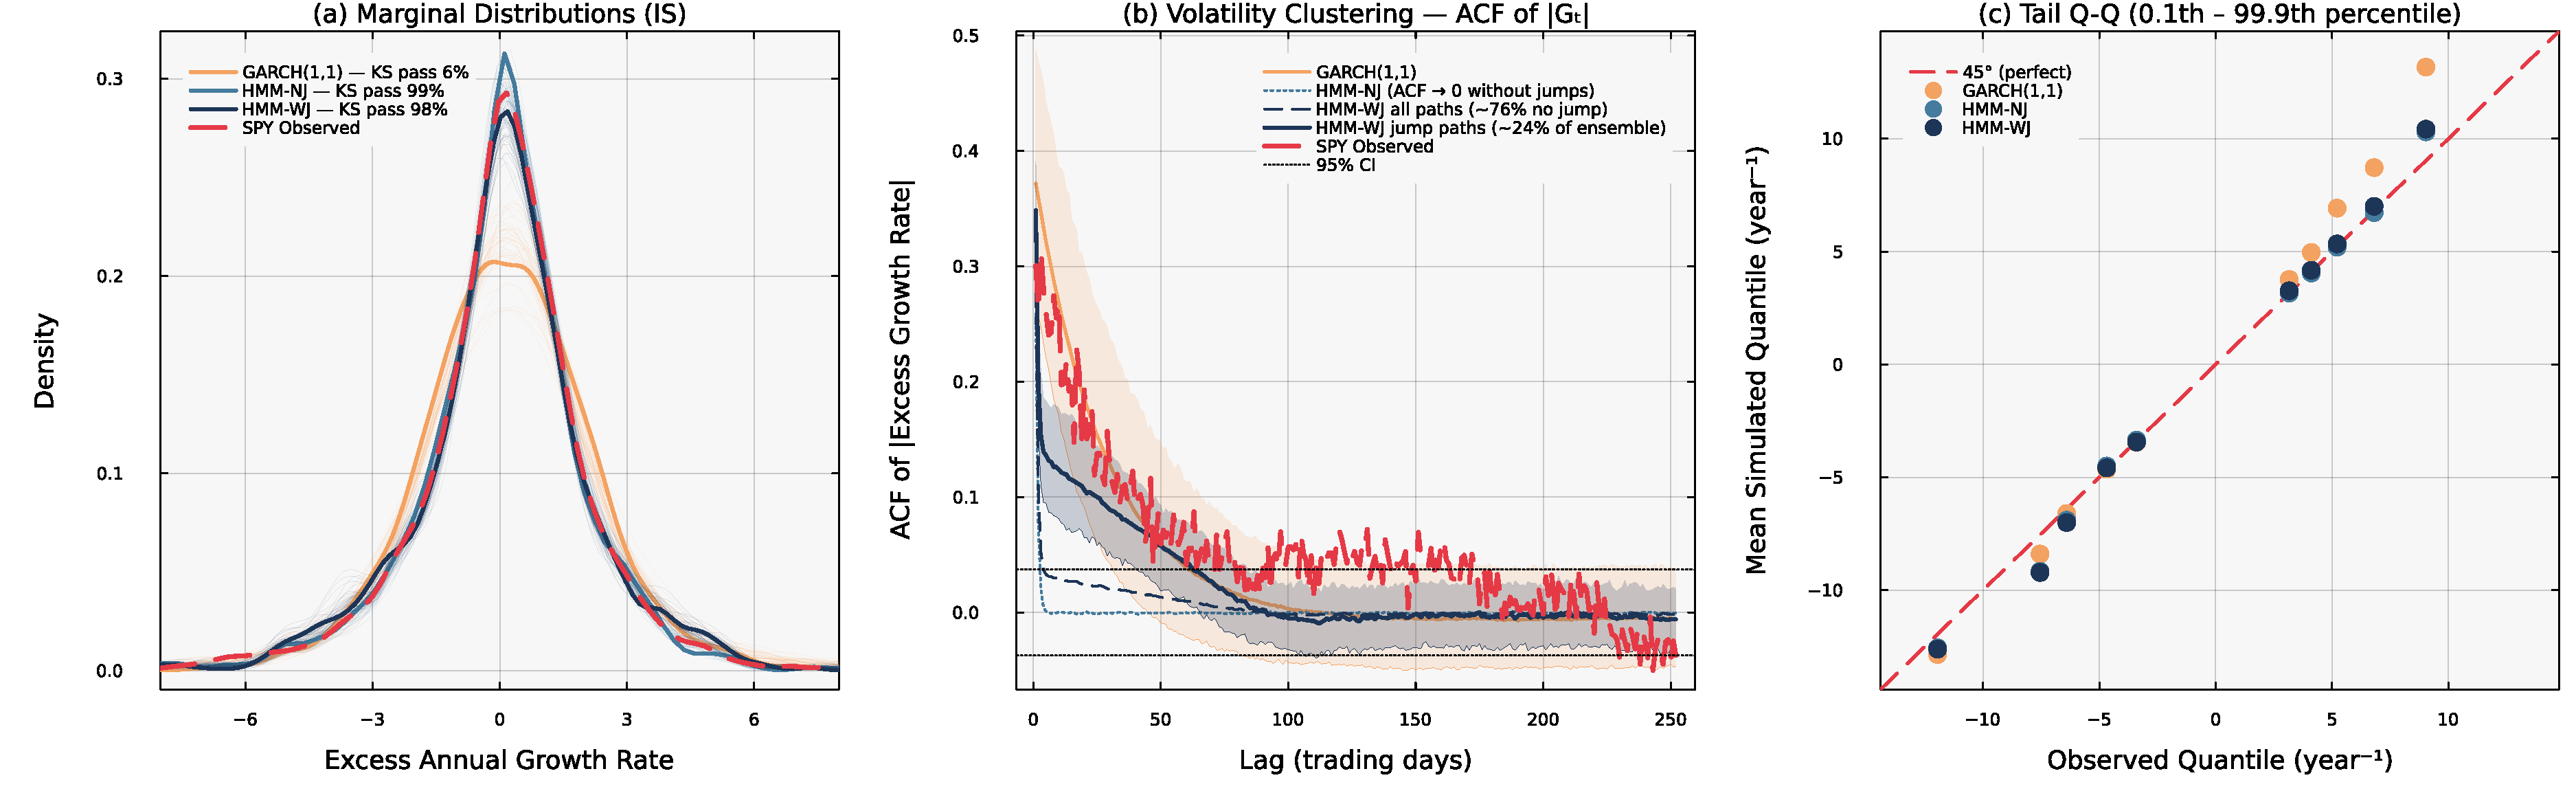
\includegraphics[width=\textwidth]{figs/main/Fig03-Model-Comparison.pdf}
  \caption{\textbf{Head-to-head in-sample model comparison for SPY}
    ($N = 100$, $1{,}000$ simulated paths). \emph{Panel (a):} marginal
    density of excess growth rates with in-sample KS pass rates
    annotated per generator. \emph{Panel
    (b):} autocorrelation function of $|G_t|$ at lags $1$--$252$
    (shaded bands: $10$th--$90$th percentile across paths) per
    generator. \emph{Panel (c):}
    tail Q-Q plot at the $0.1$st--$99.9$th percentile region per
    generator.}
  \label{fig:model_comparison}
\end{figure}

To measure how jump-active paths changed the results, we resampled the
fitted ensemble at different jump-path fractions $f$
(Figure~\ref{fig:jump_mix}). Here $f$ is the share of accepted paths
that contain at least one jump. We varied $f$ from $0$, where all
accepted paths reduce to HMM-NJ, to $1$, where every accepted path
contains a jump. This procedure held the fitted model fixed and
changed only the mixture of accepted paths. The absolute-return autocorrelation error fell monotonically
from $0.059$ at $f = 0$ to $0.037$ at $f = 1$, moving from the no-jump
value toward the GARCH value as the jump share rose. Over the
same sweep, simulated excess kurtosis declined from $7.9$ to $6.7$,
matching the observed value near $f \approx 0.14$ and falling below
it thereafter. The two-sample KS and AD pass rates also declined. The
Hill upper-tail index stayed near $0.35$, against an observed $0.32$,
across the whole sweep because the Student-$t$ ($\nu = 5$) emission
sets the tail exponent independently of jump content. Increasing the
jump share therefore traded fit to the distributional body for lower
autocorrelation error without changing the tail index.

The value
$f \approx 0.25$ used throughout kept simulated kurtosis within
$2\%$ of the observed value and lowered the autocorrelation error
about a quarter of the way from the no-jump value toward the
all-jump endpoint.
Thus, the selected mixture provided a compromise between marginal and
temporal fit before the fitted marginals were carried into the
multi-asset composition experiment.

% --- Figure: jump-mix enrichment frontier ---
\begin{figure}[tbp]
  \centering
  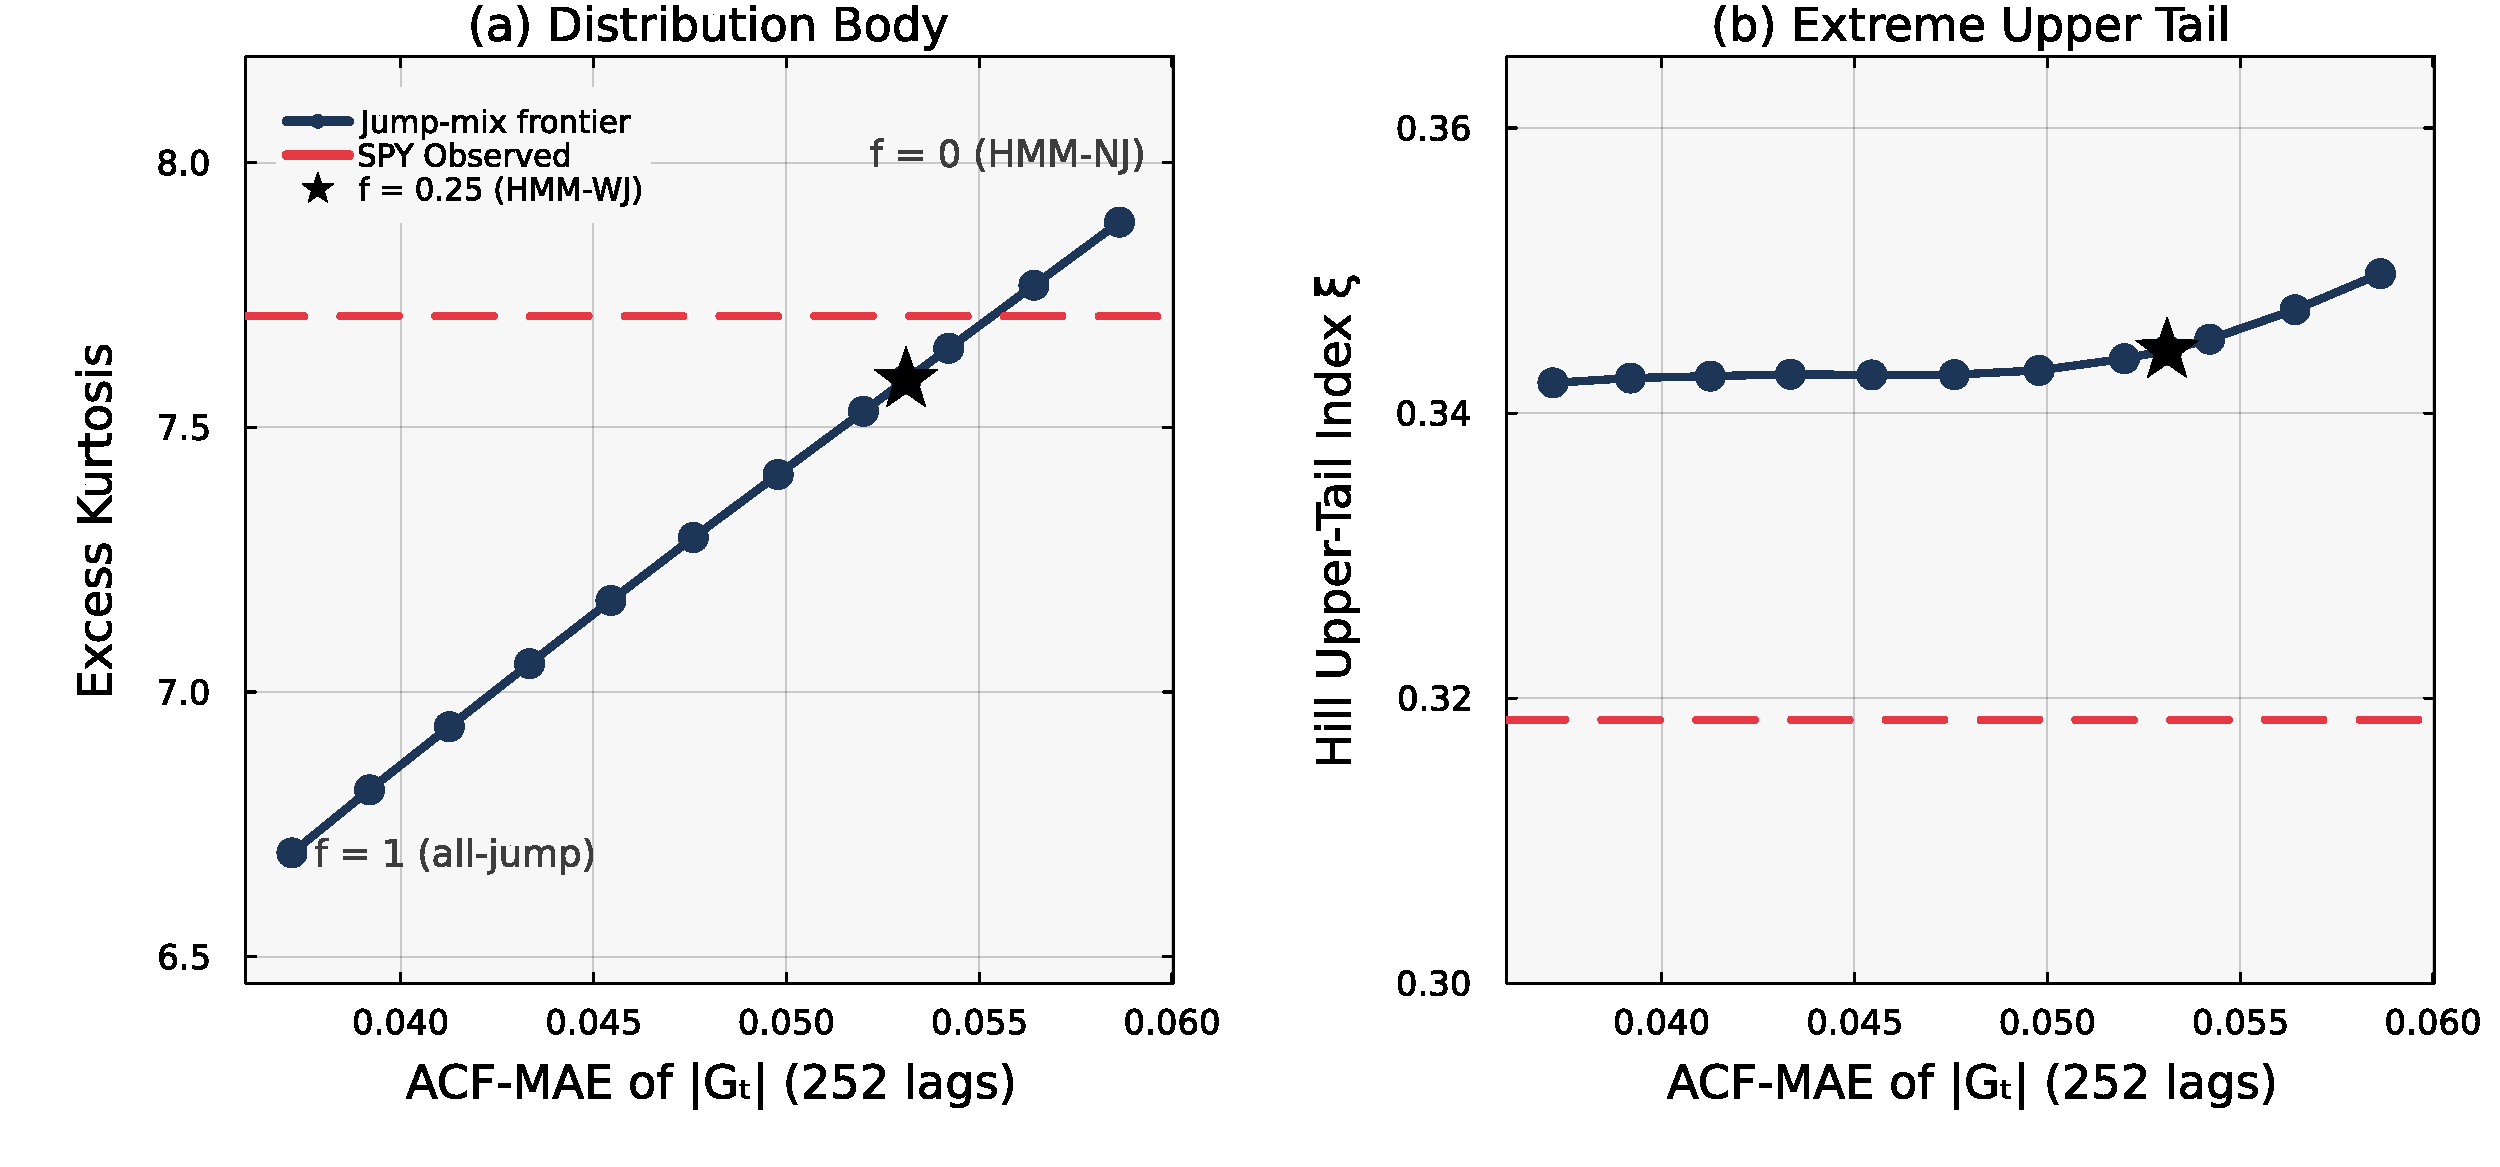
\includegraphics[width=\textwidth]{figs/main/Fig04-Jump-Mix-Frontier.pdf}
  \caption{\textbf{Jump-mix enrichment frontier for SPY} (in-sample,
    $N = 100$, pool of $4{,}000$ simulated paths). Resampling the fitted
    HMM-WJ ensemble to a target jump-path fraction $f$ (the share of
    accepted paths containing at least one jump) traces the
    temporal-marginal tradeoff. Both panels share the horizontal axis:
    absolute-return autocorrelation error (ACF-MAE of $|G_t|$ over lags
    $1$--$252$); lower values indicate stronger volatility clustering.
    Panel (a): simulated excess kurtosis. Panel (b): Hill upper-tail
    index $\xi$, the raw estimator equal to the reciprocal of the tail
    exponent. Red dashed lines mark the observed SPY values; the star
    marks the $f \approx 0.25$ value used throughout.
    Endpoints $f = 0$ and $f = 1$ correspond to the no-jump generator
    and an all-jump ensemble.}
  \label{fig:jump_mix}
\end{figure}

\subsection{Variance-corrected multi-asset composition}

The single-asset results defined the tradeoff in the marginal
generator. We then tested whether the variance-corrected SIM preserved
each asset's variance and factor loading across the $423$-ticker
universe, comparing the six composition methods on the aggregate
scorecard (Table~\ref{tab:aggregate}).
% --- Table: Aggregate scorecard across composition methods ---
\begin{table}[H]
  \centering
  \caption{\textbf{Aggregate scorecard across $423$ non-market tickers and
    $100$ replications per ticker.} Median values per composition
    method.
    $|\hat\alpha - \alpha|$, $|\hat\beta - \beta|$, and
    $|\hat R^2 - R^2_{\real}|$: absolute deviation between OLS recovery
    and calibration (intercept error has units of $\mathrm{yr}^{-1}$).
    KS pass and AD pass: fraction of
    replications whose two-sample test against the real marginal exceeds
    $p = 0.05$. $W_1$: Wasserstein-1 distance to the real marginal.
    $\kappa$: sample excess kurtosis. Hill: tail-index estimate on the
    upper $5\%$ of $|g|$.}
  \label{tab:aggregate}
  \small
  \resizebox{\textwidth}{!}{\begin{tabular}{lrrrrrrrr}
\toprule
Composer & $|\hat\alpha-\alpha|$ & $|\hat\beta-\beta|$ & $|\hat R^2 - R^2_{\real}|$ & KS pass (\%) & AD pass (\%) & $W_1$ & $\kappa$ & Hill \\
\midrule
Naive & 0.002 & 0.022 & 0.087 & 7.1 & 3.5 & 0.700 & 7.767 & 0.369 \\
Gaussian SIM & 0.048 & 0.017 & 0.008 & 0.6 & 0.5 & 0.682 & 1.427 & 0.217 \\
Hybrid & 0.002 & 0.018 & 0.021 & 73.6 & 64.6 & 0.249 & 7.165 & 0.365 \\
JumpHMM-on-residuals & 0.049 & 0.018 & 0.015 & 75.8 & 70.7 & 0.232 & 7.262 & 0.365 \\
Block bootstrap & 0.042 & 0.017 & 0.020 & 73.3 & 66.8 & 0.232 & 6.675 & 0.330 \\
GARCH(1,1)-$t$ & 0.047 & 0.017 & 0.036 & 67.4 & 61.4 & 0.267 & 6.069 & 0.317 \\
\bottomrule
\end{tabular}
}
\end{table}
All six methods recovered the factor loading with similar accuracy:
the median absolute $\beta$ error ranged from $0.018$ to $0.022$
(Table~\ref{tab:aggregate}). Path centering also kept the median
absolute intercept error at $0.002\,\mathrm{yr}^{-1}$ for both methods
that used full-return draws. The residual-fit methods retained random
variation in the residual mean over each finite path. Their larger
intercept errors therefore do not, by themselves, imply a worse fit
to the return distribution.

The larger differences appeared in variance recovery and tail
behavior. Gaussian SIM had the lowest median $R^2$ error because it
targets $R^2$ directly. However, it almost never passed the
distributional tests, and its median excess kurtosis was an order of
magnitude below the observed value (Fig.~\ref{fig:tails}). Centered
naive composition retained the shape of the full-return draw, but
adding the market factor inflated its variance by
$\beta_i^2\sigma_m^2$. The hybrid method removed that extra variance.
It passed $73.6\%$ of KS comparisons and retained heavy tails, with
median excess kurtosis of $7.2$ and a Hill index of $0.36$. Its median
$R^2$ error fell between those of the naive and Gaussian methods
because this branch preserves the generator variance rather than
targeting the observed $R^2$ directly.

The three residual-fit methods avoided double counting by fitting
their generators to the empirical OLS residuals, whose variance
already excludes the market component. Their KS pass rates ranged
from $67.4\%$ for GARCH(1,1)-$t$ to $75.8\%$ for
JumpHMM-on-residuals. The hybrid rate was two percentage points below
JumpHMM-on-residuals and slightly above block bootstrap.
JumpHMM-on-residuals and block bootstrap had slightly lower
Wasserstein distances. JumpHMM-on-residuals also matched the hybrid's
kurtosis and Hill index almost exactly, whereas the block-bootstrap
and GARCH residual fits produced lighter tails. Thus, the correction
substantially improved on naive composition and approached the best
residual-fit method without requiring a second fit for each asset. We
next tested whether this ordering persisted after all fitted
parameters were frozen.

We froze the fitted models and SIM parameters before evaluating them
against $416$ complete asset histories from $2025$
(Table~\ref{tab:oos_composition}). The hybrid
method reached an $87.0\%$ mean cross-ticker KS pass rate, against
$83.5\%$ for centered naive composition, and its median composed-to-observed
variance ratio was $0.97$, whereas naive composition remained
inflated at $1.29$. JumpHMM-on-residuals reached an $86.2\%$ KS pass
rate and a slightly lower median $W_1$ than the hybrid. Matched-length
training blocks produced lower pass rates for every method. The higher
$2025$ pass rates did not arise solely from comparing samples of
$249$ rather than $2{,}766$ observations.

The average pass rates concealed substantial differences among
tickers (Figure~\ref{fig:oos_composition}). Most ticker-level rates
were near the upper end of the range, but every method retained a
lower tail of weak fits. For the hybrid method, many tickers improved
relative to their matched-length training blocks, while a subset
deteriorated out of sample.
Thus, the held-out marginal improvement was broad but not uniform
across assets, motivating a separate check of whether the resulting
synthetic tails produced reliable risk thresholds.

\begin{table}[H]
  \centering
  \caption{\textbf{Frozen-parameter multi-asset evaluation on the
    $2025$ holdout.} Results cover $416$ non-market tickers and $100$
    replications per ticker; GARCH covers $386$ tickers. Pass rates
    are first averaged within ticker and then across tickers.
    \textit{matched IS} compares each synthetic path with a randomly
    selected contiguous $249$-day block from the $2014$--$2024$
    training history, matching the holdout sample length. $W_1$ and
    the variance ratio are medians across ticker-level medians; the
    variance ratio is synthetic variance divided by observed $2025$
    variance.}
  \label{tab:oos_composition}
  \small
  \begin{tabular}{lrrrrrr}
\toprule
 & \multicolumn{2}{c}{KS pass (\%)} & \multicolumn{2}{c}{AD pass (\%)} & & \\
\cmidrule(lr){2-3} \cmidrule(lr){4-5}
Composer & matched IS & 2025 & matched IS & 2025 & $W_1$ (2025) & variance ratio \\
\midrule
Naive & 69.4 & 83.5 & 54.8 & 71.6 & 0.877 & 1.29 \\
Gaussian SIM & 57.4 & 73.9 & 44.9 & 64.6 & 0.866 & 0.97 \\
Hybrid & 78.8 & 87.0 & 66.2 & 79.7 & 0.716 & 0.97 \\
JumpHMM-on-residuals & 77.9 & 86.2 & 65.6 & 80.1 & 0.708 & 0.98 \\
Block bootstrap & 76.3 & 84.0 & 64.0 & 76.5 & 0.715 & 0.90 \\
GARCH(1,1)-$t$ & 74.5 & 82.6 & 62.6 & 75.0 & 0.733 & 0.91 \\
\bottomrule
\end{tabular}

\end{table}

\begin{figure}[H]
  \centering
  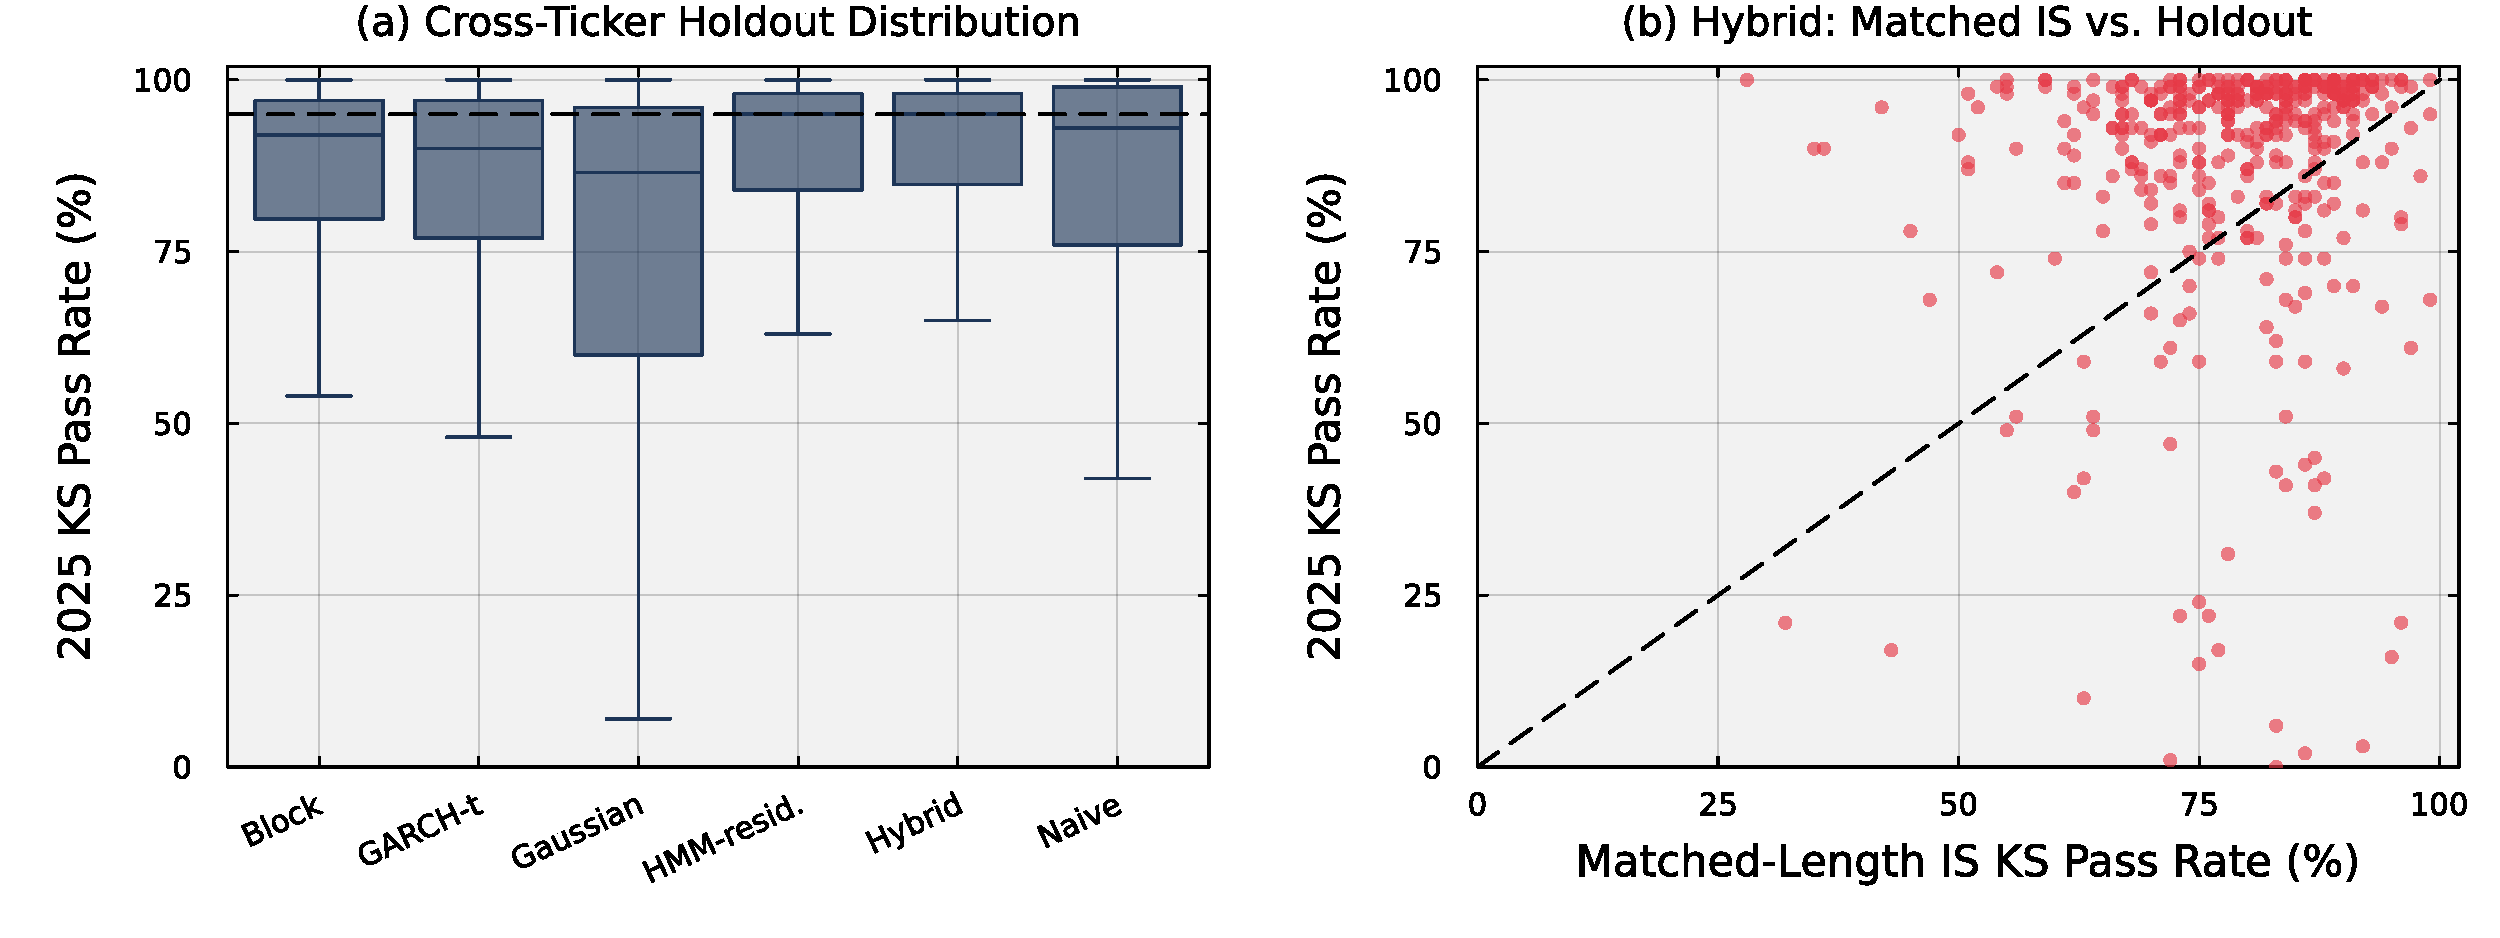
\includegraphics[width=\textwidth]{figs/main/Fig05-OoS-Composition.pdf}
  \caption{\textbf{Cross-ticker distribution of frozen-parameter
    out-of-sample marginal fit.} Panel~(a) shows the distribution of
    per-ticker $2025$ KS pass rates across $100$ replications; the
    dashed line marks $95\%$. Panel~(b) compares each ticker's hybrid
    KS pass rate against a matched-length training block with its
    pass rate against the $2025$ holdout. The diagonal denotes equal
    performance.}
  \label{fig:oos_composition}
\end{figure}
\FloatBarrier

\subsection{VaR coverage}

We used the frozen synthetic paths to estimate per-ticker one-day
Value-at-Risk (VaR) thresholds and counted exceedances on the real
$2025$ histories (Table~\ref{tab:var}). At $\alpha=0.95$, the hybrid
and JumpHMM-on-residuals methods produced mean exceedance rates of
$5.97\%$ and $6.07\%$, respectively, against the $5\%$ nominal rate.
At $\alpha=0.99$, both rates were $1.67\%$, against the
$1\%$ nominal rate. Naive composition was closest at the $99\%$
level ($1.21\%$), while Gaussian SIM had the largest exceedance rate
($2.03\%$). The short holdout contains only about $2$--$3$ expected
$99\%$ exceedances per ticker, so we interpret the corresponding
Kupiec pass rates and cross-ticker dispersion as low-power checks
rather than precise rankings.
Taken together, the VaR results showed that stronger marginal fit did
not automatically imply nominal tail coverage, motivating a closer
look at where the variance correction was most stable.

% --- Table: VaR coverage check ---
\begin{table}[H]
  \centering
  \caption{\textbf{Out-of-sample per-ticker one-day Value-at-Risk
    coverage across the six composition methods.} VaR thresholds at
    coverage level $\alpha$ were estimated from frozen-parameter
    synthetic paths and exceedances were counted against the real
    $2025$ growth-rate history. \textit{rate}: mean of the per-ticker
    mean exceedance rates (nominal: $1-\alpha$). \textit{SD}:
    cross-ticker standard deviation, in percentage points.
    \textit{Kupiec pass}: mean within-ticker fraction of replications
    whose unconditional-coverage test $p$-value exceeds $0.05$.}
  \label{tab:var}
  \small
  \setlength{\tabcolsep}{5pt}
  \begin{tabular}{lrrrrrr}
\toprule
 & \multicolumn{3}{c}{$\alpha = 0.95$} & \multicolumn{3}{c}{$\alpha = 0.99$} \\
\cmidrule(lr){2-4} \cmidrule(lr){5-7}
Composer & rate (\%) & SD (pp) & Kupiec pass (\%) & rate (\%) & SD (pp) & Kupiec pass (\%) \\
\midrule
Naive & 4.37 & 2.15 & 65.8 & 1.21 & 0.76 & 78.9 \\
Gaussian SIM & 4.95 & 2.26 & 70.0 & 2.03 & 1.17 & 72.1 \\
Hybrid & 5.97 & 2.43 & 66.3 & 1.67 & 0.93 & 73.4 \\
JumpHMM-on-residuals & 6.07 & 2.59 & 67.0 & 1.67 & 0.95 & 74.5 \\
Block bootstrap & 6.13 & 2.56 & 63.7 & 1.84 & 1.01 & 73.4 \\
GARCH(1,1)-$t$ & 5.79 & 2.47 & 62.4 & 1.80 & 1.02 & 72.0 \\
\bottomrule
\end{tabular}

\end{table}

\subsection{Sensitivity analyses}

% --- Figure: preservation mechanism ---
\begin{figure}[tbp]
  \centering
  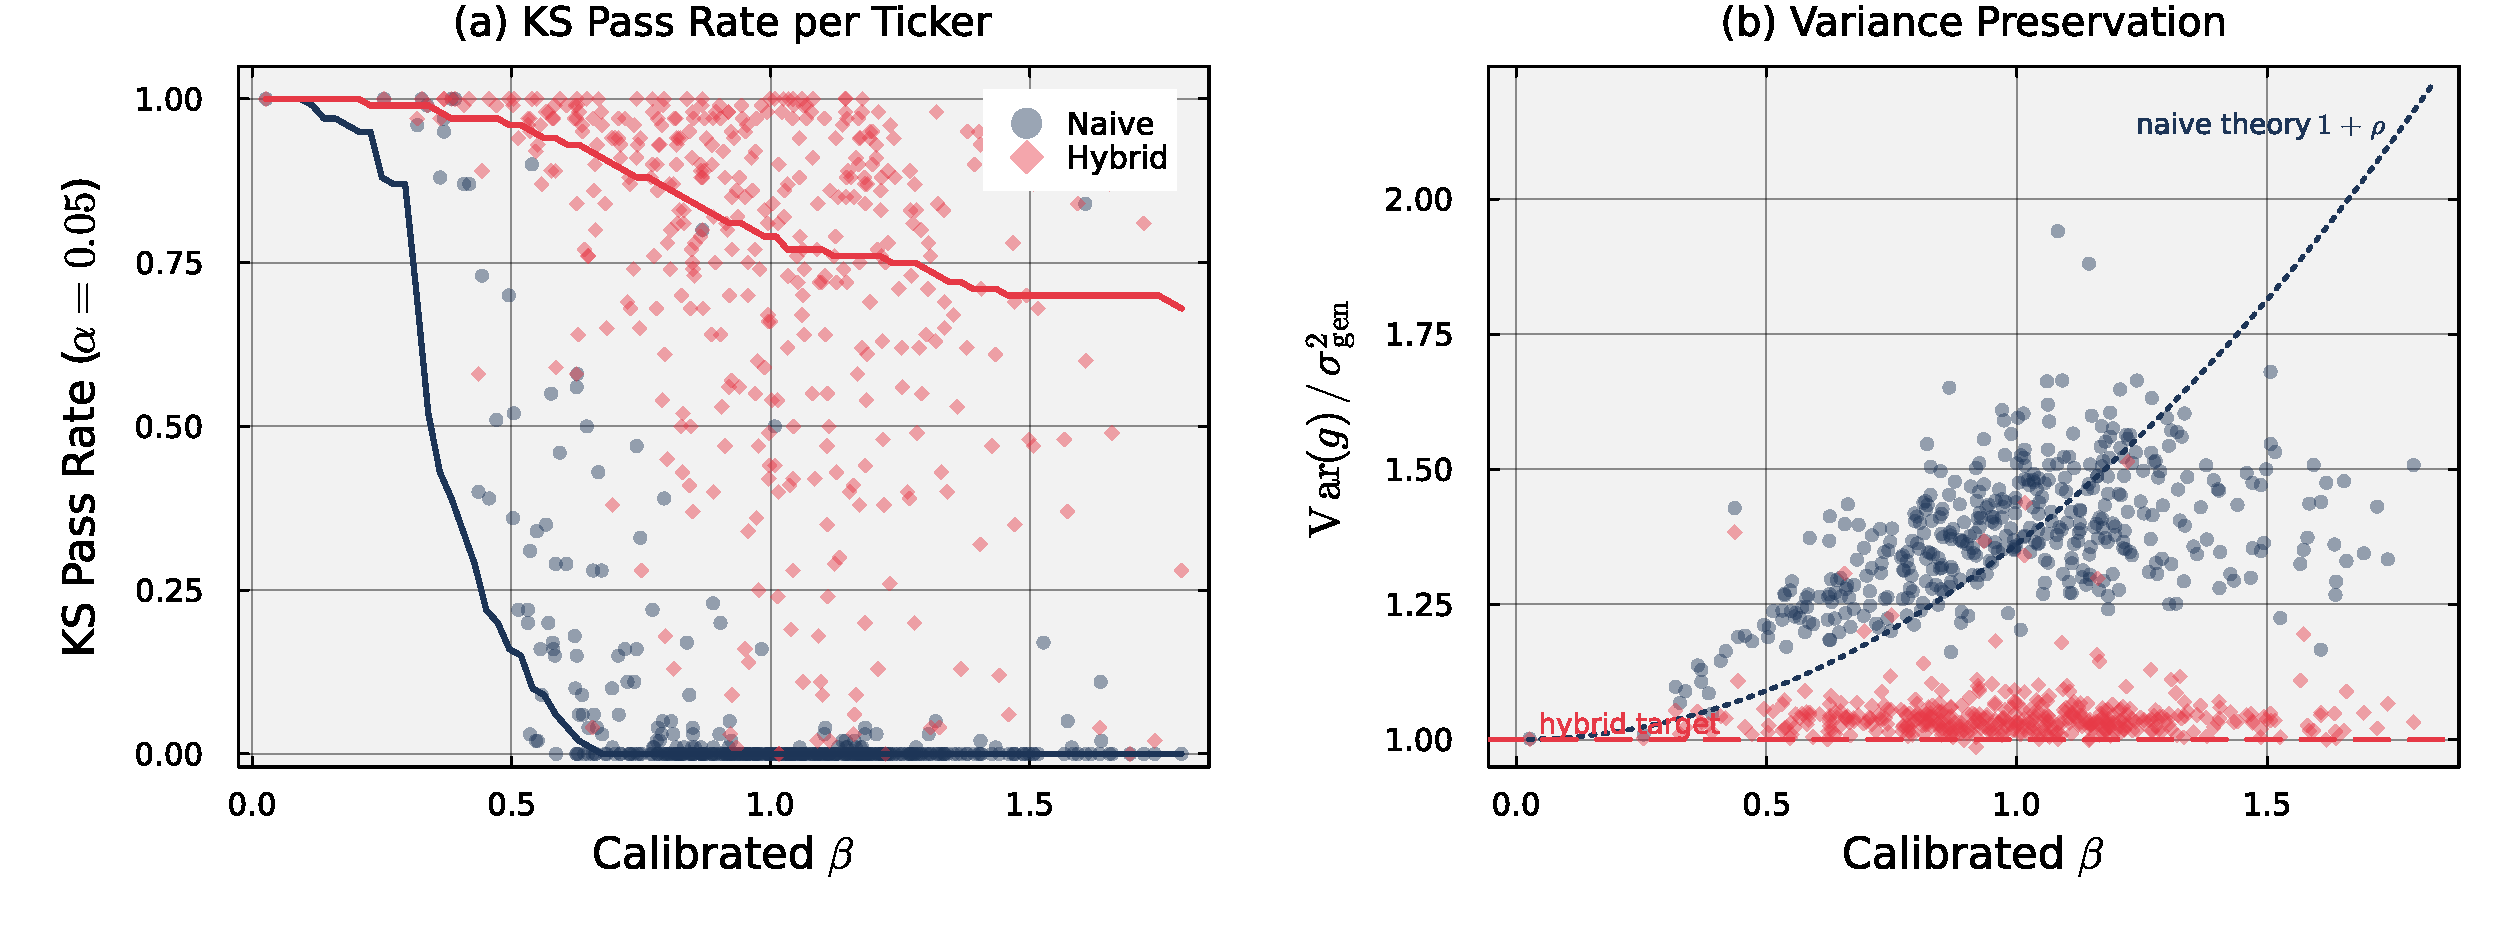
\includegraphics[width=\textwidth]{figs/main/Fig06-Variance-Preservation.pdf}
  \caption{\textbf{Hybrid's variance correction and its KS-pass-rate
    consequence, per ticker vs calibrated $\beta$.}
    Each point is a per-ticker median over $100$ replications; thick
    lines are binned medians. \emph{Left (consequence):} Kolmogorov--Smirnov
    pass rate against the real marginal at $\alpha = 0.05$ for naive
    composition (blue) and hybrid (orange).
    \emph{Right (cause):} variance ratio
    $\mathrm{Var}(g)/\sigma^2_{\mathrm{gen}}$ for the same two methods. The dotted curve is the
    theoretical naive inflation $1 + \rho$ evaluated at the universe-median
    $\sigma^2_{\mathrm{gen}}$; the dashed line marks a variance ratio of
    one.}
  \label{fig:preservation}
\end{figure}

To isolate how the variance correction changed marginal fit, we
plotted each ticker's KS pass rate and variance ratio
$\mathrm{Var}(g)/\sigma_{\gen}^2$ against its calibrated $\beta$
(Fig.~\ref{fig:preservation}). Under naive composition, the variance
ratio followed $1+\rho_i$ and exceeded generator variance by
$50$--$75\%$ at high $\beta$, and the naive KS pass rate fell toward
zero above $\beta \approx 0.7$; the hybrid method held the ratio at
one and retained substantially higher pass rates across the
$\beta$ range.

The branch-selection
rule assigned $421$ tickers to the variance-preserving branch, two
trackers to the $R^2$-preserving branch, and none to the clipped
branch (Fig.~\ref{fig:branch_map}, Table~\ref{tab:branch}). The two
$R^2$-preserving assignments were QQQ and SPYG, and both had a $100\%$
KS pass rate; the highest-$R^2$ individual stock, BLK, fell about
$0.16$ below the $R^2_{\mathrm{preserve}}=0.80$ threshold. Clipping did not occur
in the universe: $\rho_i = \beta_i^2 \sigma_m^2 / \sigma_{\gen,i}^2$
(Eq.~\eqref{eq:rho}) stayed below $1 - f = 0.90$ for every ticker.
Because the $R^2$-preserving branch contained only two tickers, we
tested it on a synthetic-tracker grid spanning
$(\beta_{\mathrm{true}}, R^2_{\mathrm{true}}) \in \{0.8, 1.0, 1.2\}
\times \{0.80, 0.85, 0.90, 0.95, 0.99\}$. Every cell passed KS.
Thus, the correction removed the observed beta-related variance
inflation. We then tested the clipping branch under conditions that
would force it to activate.

Bucketing the universe by $\beta$ quartile, the hybrid KS pass rate
fell from $87.6\%$ in the lowest quartile to $65.9\%$ in the highest
(Table~\ref{tab:beta_bucket}). As $\beta$ increased, the market term
accounted for more of the composed variance, making the marginal more
dependent on the market distribution. We tested the clipping rule
directly by rescaling the market growth-rate path by
$\gamma \in \{1, 2, 3\}$, holding the calibrated marginals fixed
(Table~\ref{tab:stress}). At $\gamma = 1$ no ticker crossed the
threshold. At $\gamma=2$ and $3$, clipping applied to $76.4\%$ and
$95.2\%$ of tickers. Thus clipping was unnecessary under observed
market variance but activated as intended when market volatility was
artificially increased. At the observed market variance, the floor
$f$ did not affect any branch assignment; varying
$R^2_{\mathrm{preserve}}$ changed only the two tracker assignments
identified above.
